\documentclass[10pt,a4paper]{report}
\usepackage[utf8]{inputenc}
\usepackage[portuguese]{babel}
\usepackage[T1]{fontenc}
\usepackage{amsmath}
\usepackage{amsfonts}
\usepackage{graphicx}
\usepackage{lmodern}
\usepackage{amssymb}
\usepackage{verbatim}
\usepackage{float}
\usepackage{minitoc}
\usepackage{amsthm}
\newtheorem{definition}{Definição}
\newtheorem{theorem}{Teorema}
\usepackage{hyperref}
\title{\LARGE{Computabilidade e Complexidade} \\ \vspace{0.5cm} \normalsize{Resumo}}
\date{}
\renewcommand{\mtctitle}{Conteúdos}

\begin{document}

\maketitle
\tableofcontents

\chapter{Modelos de Computação}
\section{Conjuntos}
Uma linguagem ou conjunto $L$ é um conjunto de palavras sobre um alfabeto $\Sigma$, que por sua vez são conjuntos ordenados de símbolos de $\Sigma$
\begin{definition}
Conjunto recursivamente enumerável ou reconhecível:\\
A linguagem A diz-se recursivamente enumerável ou reconhecível se existir uma máquina de Turing M tal que a
computação de M sobre o input w termina na configuração de aceitação se e só se w $\in$ A.
\end{definition}
\begin{definition}
Conjunto recursivo ou decidível:\\
A linguagem A diz-se recursiva ou decidível se existir uma
máquina de Turing M tal que a computação de M para
o input w termina numa configuração de aceitação sempre
que w $\in$ A e termina numa configuração de rejeição sempre que w $\notin$ A.
\end{definition}
\begin{definition}
Função computável:\\
Uma função (possivelmente parcial) f : $\Sigma^* \rightarrow \Sigma^*$ diz-
se computável se existir uma máquina de Turing M que,
para todo o input w $\in \Sigma^*$ tal que o valor de f (w) está definido, escreve f (w) na fita de output antes de aceitar; para os demais inputs, a máquina deixa a fita de output em branco e rejeita ou não para.
\end{definition}
\section{Autómatos Finitos Deterministas}
Um autómato finito determinista é um 5-tuplo $\mathcal{M} = (Q,\Sigma,\delta,q_0,F)$, em que:
\begin{itemize}
\item $Q$ é um conjunto finito de estados
\item $\Sigma$ é o alfabeto (conjunto finito de símbolos)
\item $\delta: Q \times \Sigma \rightarrow Q$ é a função de transição
\item $q_0 \in Q$ é o estado inicial
\item $F \subseteq Q$ é o conjunto dos estados de aceitação
\end{itemize}
Dado um autómato finito determinístico $\mathcal{D} = (Q,\Sigma,\delta,q_0,F)$, a função de transição $\delta$ pode estender-se recursivamente a palavras sobre $\Sigma^*$, $\delta^*: Q \times \Sigma^* \rightarrow Q$:
\begin{itemize}
\item $\forall q \in Q, \delta^*(q, \varepsilon) = q$;
\item $\forall q \in Q$, $\forall a \in \Sigma$, $\forall w \in \Sigma^*$: $\delta^* (q,wa) = \delta(\delta^*(q,w),a)$.
\end{itemize}
\subsection{Linguagem Reconhecida por um AFD}
$\mathcal{D} = (Q,\Sigma,\delta,q_0,F)$ aceita a palavra $w \in \Sigma^*$ se $\delta^*(q_0,w) \in F$. A linguagem reconhecida por $\mathcal{D}$ é o conjunto $\mathcal{L(D)} = \{w \in \Sigma^*: \mathcal{D}\; aceita\; w\}$.\\
\\
Uma linguagem diz-se regular se existe um AFD que a reconhece. A classe das linguagens regulares está fechada para a complementação, para a interseção finita e para união finita.

\section{Autómatos Finitos Não Deterministas}
Um autómato finito não determinista é um 5-tuplo $\mathcal{M} = (Q,\Sigma,\delta,q_0,F)$, em que:
\begin{itemize}
\item $Q$ é um conjunto finito de estados
\item $\Sigma$ é o alfabeto (conjunto finito de símbolos)
\item $\delta: Q \times \Sigma_\varepsilon \rightarrow \mathcal{P}(Q)$ é a função de transição, em que $\Sigma_\varepsilon = \Sigma \cup \{\varepsilon\}$
\item $q_0 \in Q$ é o estado inicial
\item $F \subseteq Q$ é o conjunto dos estados de aceitação
\end{itemize}
Dados dois estados $p$ e $q$ do autómato $\mathcal{N}$ , diz-se que $\widetilde{pq}$ é
uma trajetória-$\varepsilon$ em $\mathcal{N}$ se $\widetilde{pq}$ é uma trajetória de transições $\varepsilon$ no digrafo subjacente. Chama-se fecho-$\varepsilon$ ao conjunto de estados relativamente a um autómato $\mathcal{N}, \mathcal{E_N}: \mathcal{P}(Q) \rightarrow \mathcal{P}(Q)$, para todo $R \subseteq Q$:
$$
\mathcal{E_N} (R) = \{q \in Q: \exists r \in R, \widetilde{rq} \; \text{é uma trajetória-}\varepsilon \; \text{em} \; \mathcal{N}\}
$$
Novamente, dado um AFND $\mathcal{N} = (Q,\Sigma,\delta,q_0,F)$, a função de transição $\delta$ pode estender-se a palavras sobre $\Sigma^*, \delta^*: Q \times \Sigma^* \rightarrow \mathcal{P}(Q)$:
\begin{itemize}
\item $\forall q \in Q, \delta^*(q, \varepsilon) = \varepsilon(\{q\})$;
\item $\forall q \in Q$, $\forall a \in \Sigma$, $\forall w \in \Sigma^*$, $\delta^*(q,wa) = \bigcup_{r \in \delta^*(q,w)}\varepsilon(\delta(r,a))$.
\end{itemize}
\subsection{Linguagem Reconhecida por um AFND}
$\mathcal{N} = (Q,\Sigma,\delta,q_0,F)$ aceita $w \in \Sigma^*$ se $\delta^*(q_0,w) \cap F \neq \{\}$. A linguagem reconhecida por $\mathcal{N}$ é o conjunto $\mathcal{L(N)} = \{w \in \Sigma^*: \delta^*(q_0,w) \cap F \neq \{\}\}$.
\subsection{Converter AFND em AFD}
\begin{definition}
Dois autómatos com o mesmo alfabeto dizem-se equivalentes se reconhecem a mesma linguagem.
\end{definition}
\begin{theorem}
Todo o autómato não determinístico é equivalente a um autómato determinístico.
\end{theorem}
Seja $\mathcal{N}=(Q,\Sigma,\delta,q_0,F)$ um AFND. É possível construir um AFD $\mathcal{M}=(Q',\Sigma,\delta',q_0',F')$ tal que $L(N)=L(M)$.
\begin{itemize}
\item $Q' = \mathcal{P}(Q)$
\item $q_0' = E_\epsilon(q_0)$, i.e. o conjunto dos estados atingíveis por caminhos vazios a partir do estado inicial.
\item $\forall q' \in Q$ considere-se $R\subset Q:R = q'$. Para cada $a \in \Sigma$ definimos $\delta'(q',a) = \delta'(R,a) = \bigcup_{r\in R} E_\varepsilon(\delta(r,a)) = \{q\in Q: \exists r \in R,q \; \text{atingível por transição} \; \varepsilon \; \text{de} \; \delta(r,a)\}$
\item $F' = \{R\in Q':R \; \text{contém algum estado de aceitação de} \; \mathcal{N}\}$
\end{itemize}

\section{Máquina de Turing}
\subsection{Máquina de Turing Multi-Fita}
Uma máquina de Turing multi-fita é um 8-tuplo $MT = (Q, k, \Sigma, \Gamma, \delta, q_0, q_{aceita}, q_{rejeita})$ onde:
\begin{itemize}
\item $Q$ é um conjunto finito de estados
\item $k > 0$ é o número de fitas
\item $\Sigma$ é o alfabeto de entrada (não contém o símbolo branco)
\item $\Gamma$ é o alfabeto de fita $\Sigma \subset \Gamma$ (inclui branco)
\item $\delta: Q \times \Gamma^{k+1} \rightarrow Q \times \Gamma^{k+1} \times \{L,R,N\}^{k+2}$  é a função de transição
\item $q_0 \in Q$ é o estado inicial
\item $q_a \in Q$ é o estado de aceitação
\item $q_r \in Q$ é o estado de rejeição
\end{itemize}

\subsection{Máquina de Turing Universal}
Existe uma máquina de Turing universal $\mathcal{U}$ que:
\begin{itemize}
\item Sob o input $\mathcal{M}\star w$:
\begin{itemize}
\item Simula $\mathcal{M}_m$ sob input $n$
\end{itemize}
\end{itemize}
$$
\mathcal{U}(m\star n) \equiv \mathcal{M}_m(n)
$$
A fita da máquina universal tem o seguinte formato:
\begin{figure}[H]
\centering
\includegraphics[scale=0.3]{Sem Título.png}
\caption{Fita da MT universal}
\end{figure}
Onde:
\begin{itemize}
\item Os símbolos $Y$ delimitam a descrição de $\mathcal{M}$, em que:
\begin{itemize}
\item $X$ delimita as transições possíveis
\item $\mu_n$ representa o movimento da cabeça ($|\mu_n| = 1$, desde que apenas se considerem transições $L$ e $R$)
\item $U_n$ representa o par ($simbolo \star estado$) após a transição ($|U_n|$ é igual para todo o $n$)
\item $N_n$ representa o par ($simbolo \star estado$) antes da transição ($|N_n|$ é igual para todo o $n$ e $\forall n, k \; |N_n| = |U_k|$)
\item $W$ representa o par ($simbolo \star estado$) atual
\end{itemize}
\item $M$ representa a célula da pseudofita de $\mathcal{M}$ que está a ser visitada
\end{itemize}
Após uma fase inicial em que a cabeça de $\mathcal{U}$ é posicionada sob o último símbolo $X$, esta opera segundo 4 módulos.
\begin{figure}[H]
\centering
\includegraphics[scale=0.4]{Sem Título6.png}
\caption{Módulo inicial}
\end{figure}
\subsubsection{Módulo 1 - Encontrar Transição}
A máquina percorre a fita da direita para a esquerda, tentando encontrar o $N_n = W$. São usados os símbolos auxiliares $A$ e $B$ para marcar as transições já verificadas ($0 \rightarrow A, 1 \rightarrow B$) e $Z$, no caso de se permitir o não-movimento da cabeça.\\
\\
Termina com a cabeça a ler o símbolo á esquerda do último X.
\begin{figure}[H]
\centering
\includegraphics[scale=0.4]{Sem Título1.png}
\caption{Módulo 1}
\end{figure}
\subsubsection{Módulo 2 - Copiar Transição}
O par ($simbolo \star estado$) correspondente ao resultado da transição em curso é copiado para $W$ ($U_N \rightarrow W$). Para tal são novamente usados os símbolos $A$, $B$ e $Z$ pelo que, no final, a transição efetuada e todas á sua direita estão codificadas.\\
\\
O estado final do módulo depende do valor de $\mu_n$, que não é copiado, sendo guardado na memória do estado.
\begin{figure}[H]
\centering
\includegraphics[scale=0.4]{Sem Título2.png}
\caption{Módulo 2}
\end{figure}
\subsubsection{Módulo 3 - Restaurar $\mathcal{M}$}
No caso da cabeça da máquina não se mover, é executado o módulo 3a:\\
\\
As células com $A$, $B$ e $Z$ têm os seus valores restaurados e volta-se ao módulo 1\\
\begin{figure}[H]
\centering
\includegraphics[scale=0.5]{Sem Título3.png}
\caption{Módulo 3a}
\end{figure}
Em caso contrário executa-se o módulo 3b:\\
\\
Substitui-se o símbolo $M$ pelo sentido do movimento e, de seguida restauram-se os valores $A$, $B$ e $Z$. Por fim, escreve-se $S$ á direita do último $X$. O estado final depende do valor que estava em $S$.
\begin{figure}[H]
\centering
\includegraphics[scale=0.5]{Sem Título4.png}
\caption{Módulo 3b}
\end{figure}
\subsubsection{Módulo 4 - Mover Cabeça}
Na sequência do módulo 3b, a cabeça desloca-se até ao último $A/B$ (onde estava $M$) e troca o símbolo pelo valor que estava em $S$, guardando na memória do estado se $M$ era $A$ ou $B$. Por fim, a cabeça desloca-se no sentido do movimento, escreve $M$ e copia o seu conteúdo anterior para $S$.
\begin{figure}[H]
\centering
\includegraphics[scale=0.4]{Sem Título5.png}
\caption{Módulo 4}
\end{figure}
\subsection{Máquina de Turing Não Determinística}
A máquina de Turing não determinística corresponde a uma relaxação da computação determinística. Em qualquer momento da computação, a partir de uma mesma configuração, a máquina pode realizar transições diferentes. A única diferença reside na função de transição:
$$
\delta: Q \times \Gamma \rightarrow \mathcal{P}(Q \times \Gamma \times\{L,R,N\})
$$
Ou, no caso da máquina multi-fita:
$$
\delta: Q \times \Gamma^{k+1} \rightarrow \mathcal{P}(Q \times \Gamma^{k+1} \times\{L,R,N\}^{k+2})
$$
Cada vértice da árvore das computações relativa a uma máquina de Turing não determinística $\mathcal{M}$ e input $w$ pode ter vários descendentes, sendo o grau de ramificação limitado pela função de transição da máquina.\\
\\
Por outro lado, para toda a máquina de Turing não determinística $\mathcal{M}$ de grau de ramificação maximal $b > 2$, há sempre uma máquina não determinística $\mathcal{M}'$ de grau de ramificação maximal $b' = 2$ que lhe é equivalente. Esta transformação é conseguida escolhendo uma de entre $b$ alternativas através de uma sequência de não mais de $\lceil \log_2 b \rceil$ escolhas de 2 alternativas, atrasando-se todos os demais aspetos da computação enquanto a sequência de escolhas não estiver concluída.\\
\\
Toda a computação de profundidade $t(n)$, onde $n$ é o tamanho do input, passa a ter profundidade que não excede $\lceil \log_2 b \rceil \times t(n)$.\\
\\
Para toda a máquina de Turing não determinística $\mathcal{N}$, existe uma máquina de Turing determinística $\mathcal{D}$ que lhe é equivalente.

\chapter{Computabilidade}
\section{Silenciar uma Máquina}
\subsection{Enumeração}
Uma vez que a especificação de uma máquina de Turing é, ela mesma, uma palavra, podemos enumerar as
máquinas de Turing pela ordem lexicográfica das suas
descrições, ou qualquer outra ordem.\\
\\
Toda a enumeração de máquinas de Turing satisfaz as seguintes propriedades:
\begin{itemize}
\item[$P_1$] Para toda a máquina $\mathcal{M}$ da enumeração, existe uma máquina $\mathcal{M}^\#$ (diagonalizadora) na enumeração tal que, para todo o $n \in N, \mathcal{M}^\#$ comporta-se para com o input $n$ do mesmo modo que $\mathcal{M}$ se comporta para com o input $n\star n$.
\item[$P_2$] Para toda a máquina $\mathcal{M}$ da enumeração, existe uma máquina $\widetilde{\mathcal{M}}$ (dual) na enumeração que aceita exatamente os inputs que $\mathcal{M}$ rejeita e rejeita exatamente os inputs que $\mathcal{M}$ aceita;
\item[$P_3$] Existe na enumeração uma máquina $\mathcal{U}$, dita universal, tal que, para
todo o $m, n \in N, U$ comporta-se para com o input $m \star n$ do mesmo modo que $\mathcal{M}_m$ se comporta para com o input $n$.
\end{itemize}
Pode-se pensar em qualquer tipo de máquinas, para além das máquinas de Turing.
\subsection{Teoremas}
\begin{theorem}
Existe uma máquina $\mathcal{C}$ que, para todo o $n \in N$, processa o input $n$ exatamente da mesma maneira que a
máquina $\mathcal{M}_n$ processa o input $n$.\\
\\
Existe uma máquina $\mathcal{D}$ tal que, para todo o input n, D aceita n se $\mathcal{M}_n$ rejeita n, D rejeita n se $\mathcal{M}_n$ aceita n e D fica em silêncio se $\mathcal{M}_n$ fica em silêncio.
\end{theorem}
Toma-se para $\mathcal{C}$ a máquina $\mathcal{U}^\#$, onde $\mathcal{U}$ denota a máquina universal:
$$
\mathcal{U}^\#(n) = \mathcal{U}(n \star n) = \mathcal{M}_n(n)
$$
Pelo que $\mathcal{U}^\#$ se comporta como $\mathcal{M}_n$ sob o input $n$. Para $\mathcal{D}$ podemos tomar a máquina $\widetilde{\mathcal{U}^\#}$, uma vez que $\mathcal{D}$ é a máquina dual de $\mathcal{C}$.
\begin{theorem}
Existe um input $n$ para o qual a computação de $\mathcal{U}$ não termina.
\end{theorem}
Seja $m$ o código de $\mathcal{D} = \widetilde{\mathcal{U}^\#}$
\begin{align}
\mathcal{M}_m \; aceita \; n \; &sse \; \mathcal{D} \; aceita \; n\\
&sse \; \mathcal{U}^\# \; rejeita \; n\\
&sse \; \mathcal{U} \; rejeita \; n\star n\\
&sse \; \mathcal{M}_n \; rejeita \; n\\
seja \; &n = m\\
\mathcal{M}_m \; aceita \; m \; &sse \; \mathcal{M}_m \; rejeita \; m
\end{align}
Logo $\mathcal{M}_m$ fica em silêncio com input $m$ e $m \star m$ silencia $\mathcal{U}$
\begin{theorem}
A máquina dual da diagonalizadora da máquina $\mathcal{M}$ é a diagonalizadora da máquina dual de $\mathcal{M} (\widetilde{\mathcal{M}^\#} = \widetilde{\mathcal{M}}^\#)$.
\end{theorem}
\begin{align}
\widetilde{\mathcal{M}}^\# \; aceita / rejeita \; n \; &sse \; \widetilde{\mathcal{M}} \; aceita / rejeita \; n \star n\\
&sse \; \mathcal{M} \; rejeita / aceita \; n\star n\\
&sse \; \mathcal{M}^\# \; rejeita / aceita \; n\\
&sse \; \widetilde{\mathcal{M}^\#} \; aceita / rejeita \; n
\end{align}
\begin{theorem}
Para toda a máquina $\mathcal{M}$, existe pelo menos um input $n$ tal que $\mathcal{U}$ e $\mathcal{M}$ se comportam da mesma maneira relativamente ao input $n$.
\end{theorem}
\begin{itemize}
\item Dada uma máquina $\mathcal{M}$, seja $\mathcal{M}_m$ a máquina $\mathcal{M}^\#$;
\item Para todo o input $k$, $\mathcal{M}_m$ com input $k$ e $\mathcal{M}$ com input $k\star k$ têm o mesmo comportamento;
\item $\mathcal{U}$ com input $m\star m$ e $\mathcal{M}_m$ com input $m$ têm o mesmo comportamento;
\item Deste modo, $\mathcal{U}$ e $\mathcal{M}$ comportam-se de maneira idêntica relativamente
ao input $m\star m$;
\item Tome-se $n = m\star m$;
\end{itemize}
\begin{theorem}
Não existe uma máquina $\mathcal{M}$ que pare exatamente para os inputs que silenciam $\mathcal{U}$.
\end{theorem}
Consequência do teorema anterior:
\begin{itemize}
\item Tome-se um input $n$ relativamente ao qual as máquinas $\mathcal{U}$ e $\mathcal{M}$ concordam
\item Ambas as máquinas param dado o input $n$ ou ambas são silenciadas por $n$.
\end{itemize}

\section{Indecidibilidade}
\begin{definition}
O conjunto de aceitação $A_{TM}$ é a coleção de todos os códigos $\langle \mathcal{M}, w \rangle$, tais que $\mathcal{M}$ é uma máquina de Turing que aceita o input $w$.
$$
A = \{ m \star w : \mathcal{M}_m \; aceita \; w\}
$$
\end{definition}
\begin{definition}
O conjunto de paragem $H_{TM}$ é a coleção de todos os códigos $\langle \mathcal{M}, w\rangle$, tais que $\mathcal{M}$ é uma máquina de Turing que para (em aceitação ou rejeição) quando o input é $w$.
$$
H = \{ m \star w: \mathcal{M}_m \; aceita \; ou \; rejeita \; w\}
$$
\end{definition}
\begin{theorem}
O problema da aceitação, $\langle \mathcal{M}, w\rangle \in^? A_{TM}$, e o problema da paragem, $\langle \mathcal{M}, w\rangle \in^? H_{TM}$ são indecidíveis por uma máquina de Turing.
\end{theorem}

\begin{figure}[H]
\begin{minipage}{.5\textwidth}
\centering
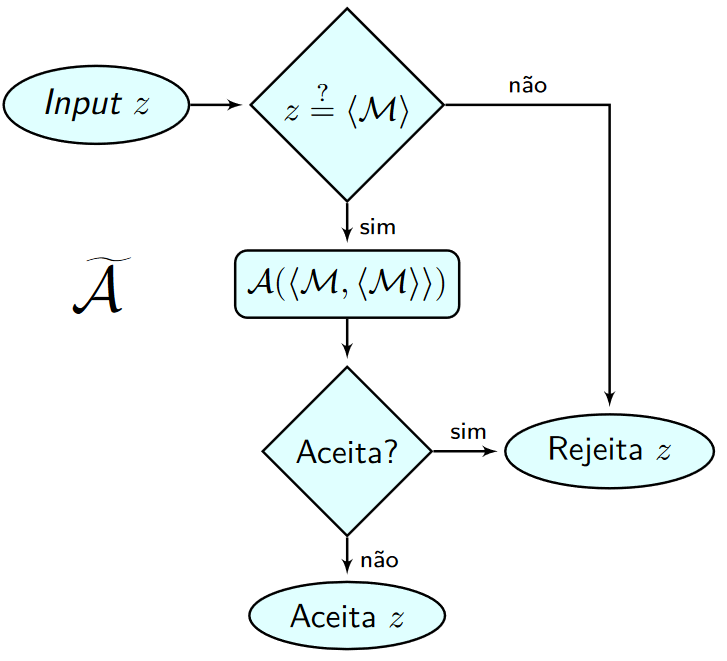
\includegraphics[width=.8\linewidth]{Sem título7.png}
\caption{Prova da indecidibilidade de $A_{TM}$. Se $\widetilde{\mathcal{A}}$ fosse construida e tivesse o seu código como input, esta aceitaria se rejeitasse e vice-versa} 
\end{minipage}%
\begin{minipage}{.5\textwidth}
\centering
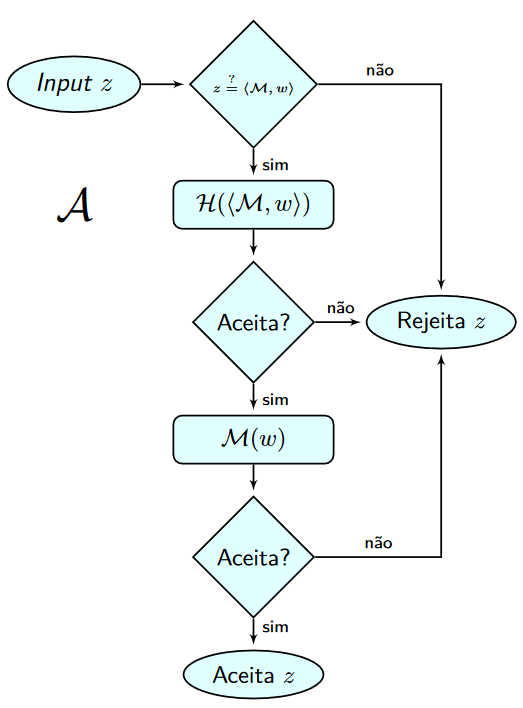
\includegraphics[width=.8\linewidth]{Sem título8.png}
\caption{Prova da indecidibilidade de $H_{TM}$. Se $\mathcal{A}$ fosse construida decidiria $A_{TM}$} 
\end{minipage}
\end{figure}

\section{Autorreferência e replicação}
Considerando uma enumeração $\mathcal{P}_1, ..., \mathcal{P}_n, ...$ de programas de construção de máquinas, associam-se respetivamente os robots $\mathcal{R}_1, ..., \mathcal{R}_n, ...$. Para todos os $x, y \in \mathbb{N}$ dizemos que o robot $\mathcal{R}_x$ constrói o robot $\mathcal{R}_y$ para significar que cada robot com o programa $\mathcal{P}_x$ constrói um robot
com o programa $\mathcal{P}_y$.\\
\\
Um robot $\mathcal{X}$ é chamado de \textit{replicante} se o robot que constrói tem o mesmo programa de $\mathcal{X}$.
\subsection{Sintaxe}
\begin{definition}
Alfabeto:\\
Seja $\Sigma$ um alfabeto cujos elementos são designados símbolos de programa. Um programa para um robot, ou simplesmente um robot, é uma palavra sobre um alfabeto $\Sigma$ que contém os símbolos notáveis $\{\mathcal{Q}, \mathcal{R}, \mathcal{C}, \mathcal{D}, \mathcal{E}, \mathcal{F}\}$.
\end{definition}
\begin{definition}
Expressões:\\
Recorremos a letras minúsculas para denotar variáveis ou expressões genéricas, as quais podem assumir qualquer valor sobre $\Sigma^*$.
\end{definition}
A ação de cada robot descrito por uma expressão $u \in \Sigma^*$ deve ser interpretada lendo $u$ da esquerda para a direita até se encontrar o operador $Q$ dito de invocação. A leitura prossegue agora da direita para a esquerda, interpretando cada um dos símbolos do alfabeto.
\begin{itemize}
\item[$\mathcal{Q}$] Para toda a expressão $x$, o programa $\mathcal{Q}x$ invoca o programa $x$.\\
Por exemplo, $\mathcal{Q}BAH$ invoca o programa $BAH$; $\mathcal{QQ}H$ invoca o programa $\mathcal{Q}H$. Porém, embora $\mathcal{Q}H$ invoque $H$, $\mathcal{QQ}H$ não invoca $H$.
\item[$\mathcal{R}$] Para todas as expressões $x$ e $y$, se $x$ invoca $y$, então $\mathcal{R}x$ invoca $yy$.\\
Por exemplo, $\mathcal{RQ}B$ invoca o programa $BB$; $\mathcal{RQ}B\mathcal{R}$ invoca o programa $B\mathcal{R}B\mathcal{R}$; para toda a expressão $x$, a expressão $\mathcal{RQ}x$ invoca $xx$. (Note-se que, em geral, $\mathcal{R}x$ não invoca $xx$.)
\item[$\mathcal{C}$] Para todas as expressões $x$ e $y$, se $x$ invoca $y$, então $\mathcal{C}x$ constrói $y$.\\
Por exemplo, $\mathcal{CQ}y$ constrói o robot $y$ (robot com o programa $y$); $\mathcal{CRQ}x$ constrói o robot $xx$; $\mathcal{CRRQ}x$ constrói o robot $xxxx$.
\item[$\mathcal{D}$] Para todas as expressões $x$ e $y$, se $x$ constrói $y$, então $\mathcal{D}x$ destrói $y$.\\
Por exemplo, $\mathcal{DCQ}x$ destrói o robot $x$ (robot com o programa $x$).
\end{itemize}
\subsection{Teoremas}
\begin{theorem} Autorreferência:\\
Existe um robot $x$ que se invoca a si mesmo, i.e. $x$ invoca $x$ ($\mathcal{RQRQ}$).
\end{theorem}
\begin{theorem}
Existe um robot $x$ tal que $\mathcal{R}x$ invoca $xx$. ($\mathcal{RQRQ}$)
\end{theorem}
\begin{theorem} Ponto fixo:\\
Dado um robot $a$, dizemos que $x$ é ponto fixo de $a$ se $x$ invoca $ax$. Todo o robot $a$ tem ponto fixo.
\begin{itemize}
\item $\mathcal{RQ}a\mathcal{RQ}$ invoca a repetição de $a\mathcal{RQ}$;
\item A repetição é $a\mathcal{RQ}a\mathcal{RQ}$
\item Ou seja ($\mathcal{RQ}a\mathcal{RQ}$) invoca $a(\mathcal{RQ}a\mathcal{RQ})$
\end{itemize}
A fórmula do ponto fixo é:
$$
\mathcal{RQ}\_\mathcal{RQ}
$$
\end{theorem}
\begin{theorem} Fórmula da criação:\\
Para todo o robot $a$, existe um robot $x$ que constrói $ax$.
\begin{itemize}
\item Procuramos um robot $y$ que invoque $a\mathcal{C}y$; consequentemente, $\mathcal{C}y$ constrói $a\mathcal{C}y$;
\item A fórmula da invocação dá-nos $y = \mathcal{RQ}a\mathcal{CRQ}$;
\item Ou seja $\mathcal{CRQ}a\mathcal{CRQ}$ constrói $a\mathcal{CRQ}a\mathcal{CRQ}$.
\end{itemize}
A fórmula da criação é:
$$
\mathcal{CRQ}\_\mathcal{CRQ}
$$
\end{theorem}
\begin{theorem} Duplo ponto fixo:\\
Existem robots $x$ e $y$ tais que $x$ invoca $ay$ e $y$ invoca $bx$.
\begin{itemize}
\item É suficiente encontrar robots $x$ e $y$ tais que $x$ invoca $a\mathcal{Q}bx$ e $y = \mathcal{Q}bx$;
\item Recorrendo à fórmula da invocação $x = \mathcal{RQ}a\mathcal{Q}b\mathcal{RQ}$ e $y = \mathcal{Q}b\mathcal{RQ}a\mathcal{Q}b\mathcal{RQ}$;
\item Alternativamente, determinamos robots $x$ e $y$ tais que $x = \mathcal{Q}ay$ e $y$ invoca $b\mathcal{Q}ay$;
\item Recorrendo de novo à fórmula da invocação obtemos $y = \mathcal{RQ}b\mathcal{Q}a\mathcal{RQ}$ e $x = \mathcal{Q}a\mathcal{RQ}b\mathcal{Q}a\mathcal{RQ}$.
\end{itemize}
\end{theorem}
\begin{theorem}
Existem robots $x$ e $y$ tais que $x$ constrói $y$ e $y$ constrói $x$.
\begin{itemize}
\item É suficiente encontrar robots $x$ e $y$ tais que $x$ constrói $\mathcal{CQ}x$ e $y = \mathcal{CQ}x$, por sua vez, constrói $x$;
\item Recorrendo à fórmula da criação $x = \mathcal{CRQCQCRQ}$ e $y = \mathcal{CQCRQCQCRQ}$.
\end{itemize}
\end{theorem}
\begin{theorem} Auto-destruição:\\
Existe um robot que se auto-destrói.

\begin{itemize}
\item Procuramos um robot $x$ que construa $\mathcal{D}x$; nestas circunstâncias o robot $\mathcal{D}x$ autodestrói-se;
\item Aplicando a fórmula da criação, $x = \mathcal{CRQDCRQ}$;
\item Ou seja, $\mathcal{DCRQDCRQ}$ autodestrói-se.
\end{itemize}
\end{theorem}
\begin{theorem} Fórmula da destruição:\\
Para todo o robot $a$, existe um robot $x$ que destrói $ax$.
\begin{itemize}
\item Procuramos um robot $x$ que construa $a\mathcal{D}x$; consequentemente, $\mathcal{D}x$ destrói $a\mathcal{D}x$;
\item A fórmula da criação dá-nos $x = \mathcal{CRQ}a\mathcal{DCRQ}$;
\item Ou seja $\mathcal{DCRQ}a\mathcal{DCRQ}$ destrói $a\mathcal{DCRQ}a\mathcal{DCRQ}$.
\end{itemize}
A fórmula da destruição é:
$$
\mathcal{DCRQ}\_\mathcal{DCRQ}
$$
\end{theorem}

\chapter{Complexidade}
\section{Funções Tempo e Espaço Construtíveis}
\begin{definition}
Função de tipo tempo:\\
Uma função total $f : \mathbb{N} \rightarrow \mathbb{N}$ diz-se própria de tipo tempo se existe uma máquina de Turing determinística $\mathcal{M}$ e um número $p \in \mathbb{N}$ tais que, para todo o input de tamanho $n \geq p, \mathcal{M}$ para exatamente ao fim de $f(n)$ transições.
\end{definition}
\begin{definition}
Função de tipo espaço:\\
Uma função total $f : \mathbb{N} \rightarrow \mathbb{N}$ diz-se própria de tipo espaço se existe uma máquina de Turing determinística $\mathcal{M}$ e um número $p \in \mathbb{N}$ tais que, para todo o input de tamanho $n \geq p, \mathcal{M}$ para numa configuração na qual exatamente $f(n)$ células são não brancas e, durante a computação, não foram lidas mais células.
\end{definition}
\subsection{Relógios}
\begin{figure}[H]
\centering
\includegraphics[scale=0.4]{Sem título10.png}
\caption{Implementação de um relógio linear numa máquina de Turing. Para input de tamanho $n$ e $k \geq 4$, efetua $kn$ transições. Para $k = 1$ a função não é construtível no tempo. Para $k = 2, 3$, podem construir-se máquinas
simplificadas}
\end{figure}
\begin{figure}[H]
\centering
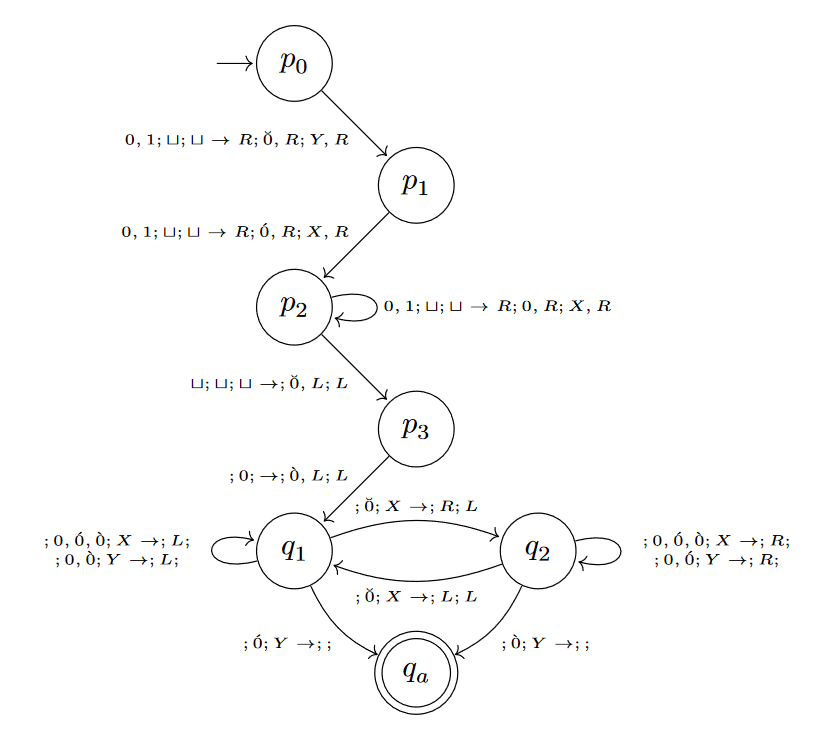
\includegraphics[scale=0.4]{Sem título9.png}
\caption{Implementação de um relógio polinomial numa máquina de Turing. Para input de tamanho $n \geq 4$, efetua $n^2$ transições.}
\end{figure}
\subsection{Construção de Uma Classe de Tempo}
Consideremos uma nova enumeração de máquinas de Turing, $\mathcal{M}_0||\mathcal{M}_t, ..., \mathcal{M}_1||\mathcal{M}_t, ..., \mathcal{M}_n||\mathcal{M}_t$ onde $\mathcal{M}_t$ é a máquina de Turing escolhida para testemunhar a construtibilidade temporal de $t(n)$, em que $n$ é o comprimento do input. $\mathcal{M}_i||\mathcal{M}_t$ é a máquina de Turing especificada como se segue:
\begin{itemize}
\item Sob input $w$ de comprimento $n$:
\begin{itemize}
\item Simula alternadamente uma transição de $\mathcal{M}_i$ e uma transição de $\mathcal{M}_t$, ambas com input $w$;
\item Se $\mathcal{M}_i$ parar primeiro, então aceita ou rejeita $w$ de acordo com $\mathcal{M}_i$; se $\mathcal{M}_t$ parar primeiro, então rejeita.
\end{itemize}
$$
DTIME(t(n)) = \{\mathcal{L}(\mathcal{M}_i||\mathcal{M}_t) : i \in \mathbb{N}\}
$$
\end{itemize}
Note-se também que a máquina $\mathcal{M}_i||\mathcal{M}_t$ pode decidir uma
linguagem diferente de $\mathcal{L}(\mathcal{M}_i)$, mesmo quando a máquina $\mathcal{M}_i$ para em todos os inputs.
\subsection{Construção de Uma Classe de Espaço}
Consideremos uma enumeração de todas as máquinas de Turing determinísticas, $\mathcal{M}_0, ..., \mathcal{M}_n, ...$, e seja $\mathcal{M}_s$ a máquina de Turing escolhida para testemunhar a construtibilidade espacial de $s$. $\mathcal{M'}_i=\mathcal{M}_s;\mathcal{M}_i$ é a máquina de Turing especificada como se segue:
\begin{itemize}
\item Sob input $w$ de comprimento $n$:
\begin{itemize}
\item Simula a computação de $\mathcal{M}_s$ e marca as primeiras $s(n)$ células da fita de trabalho;
\item Simula $\mathcal{M}_i$ nesse espaço; se esta exceder o espaço rejeita, caso contrário, tem o mesmo output que $\mathcal{M}_i$
\end{itemize}
$$
DSPACE(s(n)) = \{\mathcal{L}(\mathcal{M}_i||\mathcal{M}_s) : i \in \mathbb{N}\}
$$
\end{itemize}
\section{Decidibilidade da Paragem}
\begin{theorem}
Se $\mathcal{M}_1$ é uma máquina de Turing determinística que reconhece o conjunto $A$ em espaço próprio $s(n) \geq \log(n)$, então existe uma máquina de Turing determinística $\mathcal{M}_2$ que decide $A$ em espaço próprio $2s(n)$.
\end{theorem}
Consideremos uma máquina de Turing determinística que reconhece $A$ em espaço $s(n)$. Cada configuração da máquina é caracterizada por um estado, pelo conteúdo da fita (uma palavra sobre $\Gamma$), pela posição da cabeça de leitura/escrita da fita de trabalho e pela posição da cabeça de leitura da fita de input. Para um valor $c\in \mathbb{N}$, com $n \leq 2^{s(n)}$ seu número de configurações é majorado por:
$$
(\#Q) \times (\#\Gamma)^{s(n)} \times s(n) \times (n + 1) \leq 2^{cs(n)}
$$
Seja então $\mathcal{M}_2$ uma máquina com 3 fitas. São reservadas $s(n)$ células nas segunda e terceira fitas e simula $\mathcal{M}_1$ na segunda fita, enquanto na terceira conta o número de passos simulados.\\
\\
Se a contagem ultrapassar o número de configurações de $\mathcal{M}_1$ então esta está num ciclo infinito e $\mathcal{M}_2$ rejeita. Se $\mathcal{M}_1$ parar antes da contagem chegar ao fim, então $\mathcal{M}_2$ aceita ou rejeita, de acordo com $\mathcal{M}_2$. O espaço usado por $\mathcal{M}_2$ é $2s(n)$ para inputs de tamanho $n$.

\section{Classes de Complexidade}
Seja $f: \mathbb{N} \rightarrow \mathbb{N}_1$. Seguem-se alguns conjuntos de funções $g: \mathbb{N} \rightarrow \mathbb{N}_1$ relevantes:
\begin{align}
o(f):& \forall r \in \mathbb{R}^+, \exists p \in \mathbb{N}, \forall n \geq p: g(n) < r f(n)\\
\mathcal{O}(f):& \exists r \in \mathbb{R}^+ \exists p \in \mathbb{N}, \forall n \geq p: g(n) < r f(n)\\
\Omega_\infty(f):& \exists r \in \mathbb{R}^+ \forall p \in \mathbb{N}, \exists n \geq p: g(n) > r f(n)\\
\omega(f):& \forall r \in \mathbb{R}^+ \forall p \in \mathbb{N}, \exists n \geq p: g(n) > r f(n)\\
\Theta(f):& \exists r_1,r_2 \in \mathbb{R}^+ \exists p \in \mathbb{N}, \forall n \geq p: r_1f(n) < g(n) < r_2f(n)
\end{align}
\subsection{Tempo e Espaço}
\begin{theorem} Compressão do espaço:\\
Se o conjunto $A$ é decidível por uma máquina de Turing $\mathcal{M}$ em espaço $s$, então, para todo o $c \in \mathbb{N}_1$, existe uma
máquina de Turing $\mathcal{M}'$ que decide $A$ em espaço $\lceil \frac{1}{c}s\rceil$.
\end{theorem}
\begin{theorem} Compressão do tempo:\\
Se o conjunto $A$ é decidível por uma máquina de Turing $\mathcal{M}$ em tempo $t$, tal que $n \in o(t(n))$, então, para todo o $c \in \mathbb{N}_1$, existe uma máquina de Turing $\mathcal{M}'$ que decide $A$ em tempo $\lceil \frac{1}{c}t\rceil$.
\end{theorem}
\begin{theorem} Decidibilidade da paragem:\\
Se $\mathcal{M}_1$ é uma máquina de Turing determinística (não determinística) que reconhece o conjunto $A$ em espaço próprio $s(n) \geq \log (n)$, então existe uma máquina de Turing determinística (não determinística) $\mathcal{M}_2$ que decide $A$ em espaço próprio $s(n)$.
\end{theorem}
\begin{theorem}
Se o conjunto $A$ é decidível por uma máquina de Turing determinística $\mathcal{M}$ de $k > 2$ fitas em tempo $t(n)$, então existe uma máquina de Turing determinística de 2 fitas $\mathcal{M}'$ que decide $A$ em tempo $\mathcal{O}(t(n) \log (t(n))$.
\end{theorem}
\subsection{Classes Básicas}
Para todas as funções totais $t, s : \mathbb{N} \rightarrow \mathbb{N}$, monótonas não decrescentes, tais que $t(n) \geq n + 1$ e $s(n) \geq 1$:
\begin{itemize}
\item $DTIME(t)$ é a classe dos conjuntos decidíveis por máquinas de Turing determinísticas cujo tempo é majorado por $t$
\item $NTIME(t)$ é a classe dos conjuntos decidíveis por máquinas de Turing não determinísticas cujo tempo é majorado por $t$
\item $DSPACE(s)$ é a classe dos conjuntos decidíveis por máquinas de Turing determinísticas cujo espaço é majorado por $s$
\item $NSPACE(s)$ é a classe dos conjuntos decidíveis por máquinas de Turing não determinísticas cujo espaço é majorado por $s$
\end{itemize}
Seja $t$ um recurso de tempo e $s$ um recurso de espaço. Tem-se:
\begin{itemize}
\item $DTIME(t) \subseteq NTIME(t)$
\item $DSPACE(s) \subseteq NSPACE(s)$
\end{itemize}
Seja $t$ de acordo com a convenção para recursos de tempo e de espaço. Tem-se:
\begin{itemize}
\item $DTIME(t) \subseteq DSPACE(t)$
\item $NTIME(t) \subseteq NSPACE(t)$
\end{itemize}
Sejam $s$ e $s'$ de acordo com a convenção para recursos de espaço, $s' \in \mathcal{O}(s)$. Tem-se:
\begin{itemize}
\item $DSPACE(s') \subseteq DSPACE(s)$
\item $NSPACE(s') \subseteq NSPACE(s)$
\end{itemize}
Sejam $t$ e $t'$ de acordo com a convenção para recursos de tempo, $t'(n) \in \mathcal{O}(t(n))$ e $n \in o(t(n))$. Tem-se:
\begin{itemize}
\item $DTIME(t') \subseteq DTIME(t)$
\item $NTIME(t') \subseteq NTIME(t)$
\end{itemize}
\begin{theorem}
Se s é construtível no espaço e $s(n) \geq \log (n)$, então:
$$
NSPACE(s) \subseteq DTIME(2^{\mathcal{O}(s)})
$$
\end{theorem}
\begin{theorem}
Se t é construtível no tempo, então:
$$
NTIME(t) \subseteq DSPACE(t)
$$
\end{theorem}
\begin{theorem} Teorema de Savitch:\\
Se $s(n)$ é uma função construtível no espaço, $s(n) \geq \log (n)$ e $\mathcal{M}_1$ é uma máquina de Turing não determinística que opera em espaço $s(n)$, para inputs de tamanho $n$, e decide o conjunto $A$, então existe uma máquina de Turing determinística $\mathcal{M}_2$ que decide o conjunto $A$ e, para inputs de tamanho $n$, opera em espaço $s(n)^2$.
\end{theorem}
Uma consequência deste teorema é que:
$$
NSPACE(n^k) \subseteq DSPACE(n^{2k})
$$
\begin{theorem}Teorema de Borodin-Trakhtenbrot:\\
Para qualquer função total computável $f: \mathbb{N} \rightarrow \mathbb{N}$ tal que $f(n) \geq n, \forall n \in \mathbb{N}$, existe um limite temporal $T(N)$ tal que:
$$
DTIME(f(T(n))) = DTIME(T(n))
$$
\end{theorem}
\begin{figure}[H]
\centering
\includegraphics[scale=0.5]{Sem Título11.png}
\caption{Relações estruturais entre classes de complexidade básicas}
\end{figure}
\subsection{Classes Notáveis}
As principais classes notáveis são:
\begin{align}
LOG = &\bigcup_{k \geq 1} DSPACE(k \log(n)) = DSPACE(\log(n))\\
NLOG = &\bigcup_{k \geq 1} NSPACE(k \log(n)) = NSPACE(\log(n))\\
P = &\bigcup_{k \geq 1} DTIME(n^k)\\
NP = &\bigcup_{k \geq 1} NTIME(n^k)\\
PSPACE = &\bigcup_{k \geq 1} DSPACE(n^k)\\
NPSPACE = &\bigcup_{k \geq 1} NSPACE(n^k)\\
DEXT = &\bigcup_{k \geq 1} DTIME(2^{kn})\\
NEXT = &\bigcup_{k \geq 1} NTIME(2^{kn})\\
EXPTIME = &\bigcup_{k \geq 1} DTIME(2^{n^k})\\
NEXPTIME = &\bigcup_{k \geq 1} NTIME(2^{n^k})
\end{align}
\begin{figure}[H]
\centering
\includegraphics[scale=0.5]{Sem Título12.png}
\caption{Relações estruturais entre classes de complexidade notáveis}
\end{figure}

\subsection{Hierarquia do Espaço}
\begin{theorem}
Se $s$ e $s'$ são recursos espaciais, $s$ e $s'$ são construtíveis no espaço e $s \in o(s')$, então $DSPACE(s')$ contém um conjunto que não pertence a $DSPACE(s)$.
\end{theorem}
Outra interpretação deste resultado é que dados recursos temporais $s$ e $s'$ tais que $s' \in \omega(s)$ então:
$$
DSPACE(s') - DSPACE(s) \neq \emptyset
$$
A seguinte máquina $\mathcal{M'}$ decide um conjunto $A$ da classe $DSPACE(s')$ que não está em $DSPACE(s)$:
\begin{itemize}
\item Sob input $w$:
\begin{itemize}
\item $n = |w|$
\item Recorrendo à construtibilidade de $s'$, reservam-se $s'(n)$ células;
\item Ignora-se o prefixo da forma $1^*0$ (padding) de $w$, se este existir;
\item Verifica-se se o sufixo $u$ $(w = 1^*0u)$ codifica uma $DTM$ $\mathcal{M}_u$;
\begin{itemize}
\item Em caso afirmativo, simula-se $\mathcal{M}_u$ sobre $w$; se não rejeita-se $w$;
\end{itemize}
\item Se a simulação de $\mathcal{M}_u$ sobre $w$ for bem sucedida:
\begin{itemize}
\item Se terminar numa configuração de rejeição, então aceita-se $w$,
\item Se terminar numa configuração de aceitação, então rejeita-se $w$,
\end{itemize}
\item Se não, rejeita-se $w$.
\end{itemize}
\end{itemize}
Esta máquina opera em espaço $s'$, logo, tem-se $A \in DSPACE(s')$. \\
\\
Suponhamos que $A \in DSPACE(s)$. Seja $\mathcal{M}$ a máquina de Turing que, supostamente, decide $A$ em espaço $s$. Seja $b = \#\Gamma$ o número dos símbolos do alfabeto de trabalho de $\mathcal{M}$ e $u$ o código binário de $\mathcal{M}$.\\
\\
Como se tem $s \in o(s')$, decorre que, para uma infinidade de valores 
de $n \in N, n > |u|$, se tem que $\log(b)s(n) < s'(n)$. Note-se que $
\log(b)s(n)$ é precisamente a extensão do espaço de que $\mathcal{M'}$ 
necessita para simular $\mathcal{M}$ operando em binário (enquanto $
\mathcal{M}$ opera com um conjunto de $b$ símbolos). Tomando inputs $w$ 
da forma $1^j0u$ de tamanho $n$ ($j = n - |u| - 1$) que satisfaça a 
desigualdade anterior, $\mathcal{M'}$ tem espaço suficiente para 
completar a simulação: $w$ é aceite por $\mathcal{M'}$ se e só se é 
rejeitada por $\mathcal{M}$. Portanto, $\mathcal{M}$ não decide $A$, 
contrariamente ao pressuposto.
\begin{theorem}
Se $t$ e $t'$ são recursos temporais, $t$ e $t$ são construtíveis no tempo e $t(n) \log (t(n)) \in o(t'(n))$, então $DTIME(t')$ contém um conjunto que não pertence a $DTIME(t)$.
\end{theorem}
A seguinte máquina $\mathcal{M'}$ decide um conjunto $A$ da classe $DTIME(t')$ que não está em $DTIME(t)$:
\begin{itemize}
\item Sob input $w$:
\begin{itemize}
\item $n = |w|$
\item Inicia-se a contagem do tempo, rejeitando-se após $t'(n)$ transições no caso de a máquina não se desligar antes;
\item Ignora-se o prefixo da forma $1^*0$ (padding) de $w$, se este existir;
\item Verifica-se se o sufixo $u$ $(w = 1^*0u)$ codifica uma $DTM$ $\mathcal{M}_u$;
\begin{itemize}
\item Em caso afirmativo, simula-se $\mathcal{M}_u$ sobre $w$; se não rejeita-se $w$;
\end{itemize}
\item Se a simulação de $\mathcal{M}_u$ sobre $w$ for bem sucedida:
\begin{itemize}
\item Se terminar numa configuração de rejeição, então aceita-se $w$,
\item Se terminar numa configuração de aceitação, então rejeita-se $w$,
\end{itemize}
\item Se não, rejeita-se $w$.
\end{itemize}
\end{itemize}
Esta máquina opera em tempo $t'$, logo $A \in DTIME(t')$.\\
\\
Suponhamos que $A \in DTIME(t)$. Seja $\mathcal{M}$ a máquina de Turing que, supostamente, decide $A$ em tempo $t$. Seja $b = \#\Gamma$ o número dos símbolos do alfabeto de trabalho de
$\mathcal{M}$, $k$ o número das suas fitas e $u$ o seu código binário.\\
\\
Sabemos que uma máquina de Turing de $k > 2$ fitas pode ser simulada por uma máquina de Turing de duas fitas em tempo $ct(n) \log(t(n))$, para certa constante $c$. Como se tem $t(n) \log (t(n)) \in o(t'(n))$, decorre que, para uma infinidade de valores $n \in N, n > |u|$, se tem que $c \log(b)t(n) \log(t(n)) < t'(n)$. Note que $c \log(b)t(n) \log(t(n))$ é precisamente a extensão do tempo de que $\mathcal{M'}$ necessita para simular $\mathcal{M}$ operando em binário com duas fitas (enquanto $\mathcal{M'}$ opera com um conjunto de $b$ símbolos e $k$ fitas). Tomando inputs $w$ da forma $1^j0u$ de tamanho $n$ ($j = n - |u| - 1$) que satisfaça a desigualdade anterior, $\mathcal{M'}$ tem tempo suficiente para completar a simulação: $w$ é aceite por $\mathcal{M'}$ se e só se é rejeitada por $\mathcal{M}$. Portanto, $\mathcal{M}$ não decide $A$, contrariamente ao pressuposto.

\section{Circuitos}
\subsection{Fórmulas Booleanas}
\begin{definition} Fórmula booleana:\\
A classe das fórmulas booleanas sobre o conjunto $X$ (das variáveis) é o conjunto indutivo $BOOL_X$ definido pelas regras:
\begin{itemize}
\item Se $s \in X \cup \{0,1\}$, então $x$ é uma fórmula booleana
\item Se $F$ é uma fórmula booleana, então $\lnot F$ também
\item Se $F_1$ e $F_2$ são fórmulas booleanas, então $F_1 \land F2$ e $F_1 \lor F2$ são fórmulas booleanas
\end{itemize}
\end{definition}
\begin{definition} Fórmula booleana quantificada:\\
A classe das fórmulas booleanas quantificadas sobre o conjunto $X$ (das variáveis) é o conjunto indutivo $Q\mathbb{B}_X$ definido pelas regras:
\begin{itemize}
\item Toda a fórmula booleana é uma fórmula booleana quantificada;
\item Se $F$ é uma fórmula booleana quantificada e $x \in X$, então $\exists xF$ e $\forall xF$ são fórmulas booleanas quantificadas.
\end{itemize}
\end{definition}
\begin{definition} Atribuição de valores:\\
Uma atribuição de valores booleanos é uma aplicação $V$ de $X$ em $\{0, 1\}$. Dada uma fórmula booleana $F$ e uma atribuição de valores $V$, o valor de $F$ induzido por $V, V : BOOL_X \rightarrow \{0, 1\}$, define-se como se segue:
\begin{align}
\overline{\mathcal{V}}(F) =& \; 0 \; se \; F \; é \; 0\\
\overline{\mathcal{V}}(F) =& \; 1 \; se \; F \; é \; 1\\
\overline{\mathcal{V}}(F) =& \; \overline{\mathcal{V}}(x) \; se \; F \; é \; x, \; para \; x \in X\\
\overline{\mathcal{V}}(F) =& \; \overline{\mathcal{V}}(F_1) \times \overline{\mathcal{V}}(F_2) \; se \; F \; é \; (F_1 \land F_2)\\
\overline{\mathcal{V}}(F) =& \; \overline{\mathcal{V}}(F_1) + \overline{\mathcal{V}}(F_2) - \overline{\mathcal{V}}(F_1) \times \overline{\mathcal{V}}(F_2) \; se \; F \; é \; (F_1 \lor F_2)\\
\overline{\mathcal{V}}(F) =& \; 1 - \overline{\mathcal{V}}(F_1) \; se \; F \; é \; (\lnot F)\\
\overline{\mathcal{V}}(F) =& \; 1 - \overline{\mathcal{V}}(F_1|_{x := 0} \lor F_1|_{x := 1}) \; se \; F \; é \; (\exists xF_1)\\
\overline{\mathcal{V}}(F) =& \; 1 - \overline{\mathcal{V}}(F_1|_{x := 0} \land F_1|_{x := 1}) \; se \; F \; é \; (\forall xF_1)
\end{align}
\end{definition}
Dada uma fórmula booleana $F$ , dizemos que uma atribuição de valores $V$ satisfaz $F$ se $\overline{\mathcal{V}}(F) = 1$. Uma fórmula $F$ diz-se satisfazível se existir uma
atribuição de valores $V$ que satisfaz $F$, caso contrário, $F$ diz-se não satisfazível.\\
\\
Duas fórmulas booleanas sobre $X$, $F_1$ e $F_2$, dizem-se equivalentes, $(F_1 \equiv F_2)$, se, para toda a atribuição de valores $\mathcal{V} : X \rightarrow \{0, 1\}$, se verifica $\overline{\mathcal{V}}(F_1) = \overline{\mathcal{V}}(F_2)$.\\
\\
Suponhamos que as fórmulas booleanas sobre $X$ estão codificadas em palavras sobre $\{0, 1\}$. Eis algumas linguagens importantes:
\begin{itemize}
\item $SAT$ é o conjunto das codificações das fórmulas booleanas satisfazíveis
\item $CNF-SAT$ é o conjunto das codificações das fórmulas booleanas satisfazíveis na forma normal conjuntiva
\item $QBF$ é o conjunto das codificações das fórmulas booleanas quantificadas, sem variáveis livres, às quais corresponde o valor 1.
\end{itemize}
\subsection{Circuitos Clássicos}
Um circuito diz-se booleano, ou clássico, se todas as suas unidades lógicas de computação têm não mais do que dois inputs.
\begin{definition} Unidade de computação:\\
Uma unidade de computação sobre o conjunto (de variáveis) $X = \{x_1, . . . , x_n\}$ define-se indutivamente como se segue:
\begin{itemize}
\item Todo o elemento de $X$ é uma unidade de computação sobre $X$
\item As constantes 0 e 1 de $\mathbb{B}$ são unidades de computação sobre $X$
\item Se $g$ é uma unidade de computação sobre $X$, então $(NOT, g)$ também é uma unidade de computação sobre $X$
\item Se $g_1$ e $g_2$ são unidades de computação sobre $X$, então $(AND, g_1, g_2)$ e $(OR, g_1, g_2)$ também são unidades de computação sobre $X$
\end{itemize}
\end{definition}
\begin{definition} Sequência de computação:\\
Uma sequência de computação sobre $X$ é uma sequência $g_1, ..., g_s$, na qual cada $g_i, 1 \leq i \leq s$, é uma variável de $X$, 0 ou 1, um par $(NOT, g_l)$, com $1 \leq l < i$, um terno $(AND, g_l, g_m)$, com $1 \leq l, m < i$, ou um terno $(OR, g_l, g_m)$, com $1 \leq l, m < i$.
\end{definition}
A função de valoração $val$ do conjunto das portas e elementos fonte para o conjunto $BOOL_X$ define-se recursivamente de modo seguinte:
\[ 
val(g_i) = \left\{
\begin{array}{ll}
      g_i &se \; g_i \; é \; fonte \\
      (\lnot val (g_l)) &se \; g_i \; é \; (NOT,g_l)\\
      (val(g_l) \land val(g_m)) &se \; g_i \; é \; (AND,g_l,g_m)\\
      (val(g_l) \lor val(g_m)) &se \; g_i \; é \; (OR,g_l,g_m)
\end{array} 
\right. 
\]
Dada uma função booleana $f : \mathbb{B}^n \rightarrow \mathbb{B}^m$ (que pode ser representada por um $m$-tuplo $(f_1, . . . , f_m)$ de funções booleanas $f_i : \mathbb{B}^n \rightarrow \mathbb{B}, i = 1..m)$, dizemos que a função $f$ é computada pela sequência de computação $g_1, . . . , g_s$ se, para todo o $r, 1 \leq r \leq m$, existe $k, 1 \leq k \leq s$, tais que $f_r = val(g_k)$.
\begin{theorem}
Toda a função booleana pode ser computada por um circuito booleano clássico.
\end{theorem}
\begin{theorem}
Se $C_1$ e $C_2$ são dois circuitos booleanos que representam as expressões booleanas $\alpha_1 = \alpha_1(_x1, ..., x_n)$ e $\alpha_2 = \alpha_2(x_1, ..., x_n)$, então $C_1$ e $C_2$ são equivalentes se e só se $\alpha_1 \equiv \alpha_2$.
\end{theorem}
\subsubsection{Propriedades de Circuitos}
\begin{definition} Custo de circuitos:\\
O custo ou tamanho de um circuito é o número das suas portas. Dada uma função booleana $f$, o seu custo booleano $s_f$ , é o tamanho do mais pequeno circuito que determina os valores de $f$.
\end{definition}
\begin{definition} Profundidade de circuitos:\\
A profundidade de um circuito é o comprimento da maior trajetória no grafo do circuito. Dada uma função booleana $f$, denotamos por $d_f$ a sua profundidade booleana, i.e., a mais pequena profundidade de entre as profundidades dos circuitos que determinam os valores de $f$.
\end{definition}
\begin{definition} Complexidade:\\
Para cada $n$, definimos a complexidade do conjunto $A$, $c_A(n)$, como o custo booleano da função característica $\mathcal{X}^n_A$ de $A \cup \mathbb{B}^n$. Definimos a profundidade de $A$, $d_A(n)$, como a profundidade booleana de $\mathcal{X}^n_A$.
\end{definition}
\subsection{Circuitos $AND-OR$}
Este tipo de circuito difere dos circuitos clássicos no sentido em que vértices têm grau arbitrário. Todos os circuitos clássicos, aqueles cujas portas têm grau menor ou igual a 2, são também, circuitos $AND-OR$.
\begin{theorem}
Todo o circuito AND-OR de n inputs, custo s e profundidade d é equivalente a um circuito AND-OR de custo não superior 2s + n e profundidade não superior a d, tal que todas as portas NOT se encontram no nível 1.
\end{theorem}
\subsubsection{Codificação}
O número de inputs $x$ é codificado em unário através da palavra com $n$ uns e corresponde ao mesmo número de inputs complementares $x$, ordenados na sequência $x_1, \overline{x}_1, . . ., x_n, \overline{x}_n$.\\
\\
Para todo o $j = 1..n$, a porta $g_i \in V$ é codificada numa palavra binária de $2n + i + 2$ bits:
$$
\alpha_1\alpha_2\alpha_3\beta_1\gamma_1...\beta_n\gamma_n\delta_1...\delta_{i-1}
$$
Onde os três primeiros bits designam a porta:
\begin{itemize}
\item 001 se $l(g_i) = AND$
\item 010 se $l(g_i) = OR$
\item 000 se $l(g_i) = 0$
\item 011 se $l(g_i) = 1$
\end{itemize}
Os $2n$ bits seguintes codificam as conexões de cada um dos inputs a $g_i$:
\begin{itemize}
\item Para todo o $j = 1..n$, $\beta_j = 1$ sse $(x_j,g_i) \in E$
\item Para todo o $j = 1..n$, $\gamma_j = 1$ sse $(\overline{x}_j,g_i) \in E$
\end{itemize}
Os bits restantes codificam as ligações das portas $g_1, ..., g_{i-1}$ a $g_i$:
\begin{itemize}
\item Para todo o $j = 1..i - 1, (g_j, g_i) \in E$ se e só se $\delta_j = 1$
\end{itemize}
Um output $y$ é codificado pela palavra
$$
101 \; 00...00 \; \delta_1...\delta_m
$$
Onde $00...00$ corresponde a $2n$ zeros e, para todo o $j = 1..m, g_j \in Y$ sse $\delta_j = 1$.
\begin{figure}[H]
\centering
\includegraphics[scale=0.35]{Sem Título13.png}
\caption{Exemplo de codificação de um circuito}
\end{figure}
\subsection{Teoria do Custo de Circuitos}
\begin{theorem} Teorema do custo:\\
Existe uma função booleana $f: \mathbb{B}^n \rightarrow \mathbb{B}$ que só pode ser computada por um circuito $AND-OR$ alternado de custo $\Omega(2^{n/2})$.
\end{theorem}
Seja $\mathcal{N}(m, n)$ o número de circuitos de $n$ inputs e custo $m$. Existem $2^{m(m-1)}$ grafos orientados de $m$ vértices e $3^{nm}$ maneiras diferentes de ligar cada um destes circuitos aos $n$ inputs, pois cada vértice pode ser ligado a $x_i, \overline{x_i}$, ou a nenhum destes inputs, $1 \leq i \leq n$. Existem também $m$ maneiras de escolher a porta de output e $2^m$ maneiras de escolher a função de cada vértice. Conclui-se que $\mathcal{N}(m,n) \leq m2^{m^2}3^{nm}$.\\
\\
Existem $2^{2^n}$ funções booleanas de $n$ inputs. Se todas pudessem ser computadas por um circuito de $m$ portas, então $\mathcal{N}(m,n) \geq 2^{2^n}$. Não pode dar-se o caso de ser $m \leq n$, caso contrário a primeira desigualdade dar-nos-ia $\mathcal{N}(m, n) \leq 2^{\mathcal{O}(n^2)}$ em contradição com a segunda desigualdade. Ter-se-á então $m \geq n$. A primeira desigualdade reduz-se a $\mathcal{N}(m, n) \leq 2^{\mathcal{O}(m^2)}$, donde se conclui que $2^{\mathcal{O}(m^2)} \geq 2^{2^n}$, i.e., $m \in \Omega(2^{n/2})$.
\begin{theorem} Teorema de Riordan and Shannon:\\
Para $n \in \mathbb{N}$ suficientemente grande, existem funções booleanas de $n$ inputs de custo não inferior a $2^n / n$.
\end{theorem}
Consideremos as funções booleanas de $n$ inputs $f$ de custo $s_f \leq g(n) > n$. Podemos construir uma extensão do circuito de $f$ de forma a que o seu custo seja exatamente $g(n)$, onde $C_1$ é um circuito que computa os valores de $f$ de custo $s_f$ e $C_2$ é um circuito inútil de tamanho $g(n)-s_f$.
\begin{figure}[H]
\centering
\includegraphics[scale=0.5]{Sem Título17.png}
\caption{Ilustração do circuito auxiliar}
\end{figure}
Cada uma destas sequências de computação é constituída por $g(n)$ ternos de entre no máximo $3(g(n) + n)^2$ ternos possíveis. Ao todo, temos, no máximo, $(3(g(n) + n)^2)^{g(n)}$ sequências de computação que podem ser particionadas em classes. Certas classes consistem numa sequência que corresponde a um circuito conjuntamente com $g(n)!-1$ sequências que correspondem às possíveis permutações dos ternos. Seja $H_g(n)$ o número de funções booleanas que podem ser sintetizadas com exatamente $g(n)$ portas:
\begin{align}
H_g(n) &< \frac{1}{g(n)!}(3(g(n)+n)^2)^{g(n)}\\
&\gtrsim \frac{(12e)^{g(n)}g(n)^{2g(n)}}{g(n)^{g(n)}}\\
&< (12e)^{g(n)}g(n)^{g(n)}
\end{align}
Tomamos agora $g(n) = 2^n/n$, donde decorre que $g(n) > n, n > 4$, e, para valores de $n$ suficientemente grandes, temos:
$$
H_g(n) < (12e)^\frac{2^n}{n} \left(\frac{2^n}{n}\right)^{\frac{2^n}{n}} < (2^n)^{\frac{2^n}{n}} = 2^{2^n}
$$
\subsection{Circuitos de Custo Exponencial}
\begin{theorem}
Todo o circuito alternado de profundidade 2 que compute a função $PARITY$ tem custo pelo menos $2^{n-1} + 1$.
\end{theorem}
Consideremos um circuito $C$ de profundidade 2 que compute a função $PARITY$ tal que o nível 1 consta de portas $AND$ e o segundo nível consiste numa única porta $OR$. Deve existir no nível 1 pelo menos uma porta $AND$ cujos inputs são um subconjunto de $x_1[\alpha_1], ..., x_n[\alpha_n]$. Suponhamos que a porta $X$ tem inputs neste conjunto e, sem perda de generalidade, $X$ computa:
$$
x_1[\alpha_1] \land ... \land x_{n-1}[\alpha_{n-1}]
$$
Assim $C$ dá output 1 para ambos os inputs $(\alpha_1, ..., \alpha_{n-1}, \alpha_n)$ e $(\alpha_1, ..., \alpha_{n-1}, \overline{\alpha_n})$, o que é absurdo. Assim, a porta $X$ deve ter como inputs todos os valores $x_1[\alpha_1], ..., x_n[\alpha_n]$. Cada porta $AND$ do nível 1 deve ser específica de uma só possível palavra de $PARITY$. Conclui-se que existem $2^{n-1}$ portas no nível 1 e $2^{n-1} + 1$ portas em todo o circuito.
\begin{theorem}
Para toda a função $f: \mathbb{B}^n \rightarrow \mathbb{B}, (n > 0)$, existe um circuito $AND-OR$ alternado de custo quando muito $2^{n-1} + 1$ e profundidade 2 que computa $f$.
\end{theorem}
Se a função $f$ for constante, então é implementada com um circuito de custo 0. Suponhamos, pois, que $f$ não é constante. Um circuito alternado possível para $f$ pode ser construído através da tabela de verdade da função $f$. Consideremos os $m \in \mathbb{N}$ inputs que tornam $f$ igual a 1:
$$
(\alpha_{1,1}, ..., \alpha_{n,1}), ..., (\alpha_{1,m}, ..., \alpha_{n,m})
$$
E os $2^n - m$ inputs que tornam $f$ igual a 0:
$$
(\beta_{1,1}, ..., \beta_{n,1}), ..., (\beta_{1,m'}, ..., \beta_{n,m'})
$$
Suponhamos primeiro que $m \leq 2^{n-1}$. Podemos escrever a expressão de $f$ na forma:
$$
f(x_1, ..., x_n) = (x_1[\alpha_{1,1}] \land ... \land x_n[\alpha_{n,1}]) \lor ... \lor (x_1[\alpha_{1,m}] \land ... \land x_n[\alpha_{n,m}])
$$
Onde por $x_i[\xi]$ denota-se $x_i$ se $\xi = 1$ e $\overline{x_i}$ se $\xi = 0$, para todo o $1 \leq i \leq n$. Deste modo, a função $f$ pode ser computada por um circuito alternado de profundidade 2 cujo nível 1 é constituído por portas $AND$ e o nível 2 consiste numa única porta $OR$ com inputs de todas as portas $AND$ do nível 1. O custo deste circuito é $m + 1 \leq 2^{n-1} + 1$. Suponhamos agora que $m \geq 2^{n-1}$. Neste caso operamos com os inputs que dão valor 0 a $f$:
$$
f(x_1, ..., x_n) = (\overline{x_1}[\beta_{1,1}] \lor ... \lor \overline{x_n}[\beta_{n,1}]) \land ... \land (\overline{x_1}[\beta_{1,m'}] \lor ... \lor \overline{x_n}[\beta_{n,m'}])
$$
De novo se conclui que $f$ pode ser computada por um circuito alternado cujo nível 1 é constituído por $m'$ portas $OR$ e o nível 2 consiste numa única porta $AND$ com inputs provenientes de todas as portas $OR$. Este circuito tem custo $m' + 1 \leq 2^{n-1} + 1$.
\begin{theorem}
Qualquer função $f: \mathbb{B}^n \rightarrow \mathbb{B}$ que pode ser computada por um circuito alternado de profundidade 2 com $p$ portas $AND$ de $n$ inputs no nível 1 e 1 porta $OR$ no nível 2, pode ser computada por um circuito alternado de profundidade 2 e custo $n^p + 1$, com portas $OR$ no nível 1 e 1 porta $AND$ no nível 2. Este resultado é válido se trocarmos as portas $AND$ por portas $OR$.
\end{theorem}
\begin{figure}[H]
\centering
\includegraphics[scale=0.32]{Sem Título14.png}
\caption{Ilustração da conversão $AND-OR$ para $OR-AND$}
\end{figure}
\begin{theorem}
Toda a função $f: \mathbb{B}^n \rightarrow \mathbb{B}$ pode ser computada por um circuito $AND-OR$ alternado de custo $\mathcal{O}(2^{n/2})$ e profundidade 3.
\end{theorem}
\begin{figure}[H]
\centering
\includegraphics[scale=0.5]{Sem Título15.png}
\end{figure}
\begin{figure}[H]
\centering
\includegraphics[scale=0.5]{Sem Título16.png}
\caption{Ilustração da construção de um circuito simplificado para $f$. É usada uma função $g(x_1,x_2)$ auxiliar que tem como valor as combinações de $x_3$ e $x_4$ que tornam $f$ verdadeira. Por exemplo, $g(0,0) = (\overline{x_3} \land \overline{x_4}) \lor (x_3 \land \overline{x_4}) \lor (x_3 \land x_4)$}
\end{figure}
\subsection{Simulação de Máquinas de Turing}
Consideremos uma máquina de Turing determinística $\mathcal{M}$ de apenas uma fita, alfabeto de trabalho $\Gamma = \{a_1, ..., a_n\}$, conjunto de estados $Q = \{q_1, ..., q_m\}$ e função de transição $\delta: Q \times \Gamma \rightarrow Q \times \Gamma \times \{L, R, N\}$.\\
\\
Seja $r = \lceil \log |Q| \rceil + 1$ e $r' = \lceil \log |\Gamma| \rceil + 1$. Codificamos os estados de $Q$ em binário através de sequências de $r$ bits, excluindo a sequência $0^r$. Similarmente, codificamos os símbolos de $\Gamma$ em binário como sequências de $r'$ bits, excluindo a sequência $0^{r'}$.\\
\\
Em cada passo da computação de $\mathcal{M}$, associamos a cada célula $u$ da fita de $\mathcal{M}$ uma representação dos seus parâmetros: o conteúdo da célula, se a cabeça de leitura/escrita está posicionada ou não nessa célula e, em caso afirmativo, o estado de $\mathcal{M}$ nessa configuração. Esta representação é dada através de um par $u_i = (e_i, x_i)$, onde $x_i$ é o código do símbolo que ocupa a célula $u$ ao fim de $i$ transições e $e_i$ é o código do estado da máquina ao fim de $i$ transições, definido por:
\[ 
e_i = \left\{
\begin{array}{ll}
      0^r &se \; \mathcal{M} \; não \; se \; encontra \; em \; u \; ao \; fim \; de \; i \; transições\\
      código \; de \; q_l &se \; \mathcal{M} \; se \; encontra \; em \; u \; no \; estado \; q_i \; ao \; fim \; de \; i \; transições
\end{array} 
\right. 
\]
Suponhamos que, quando $\mathcal{M}$ entra no estado de aceitação $q_a$, aí permanece em ciclo até terem sido completadas as $t(n)$ transições. Construímos um circuito booleano que simula a evolução do conteúdo da fita de $\mathcal{M}$ quando o input é $w$, impresso nas $|w|$ células mais à esquerda da fita de $\mathcal{M}$, durante exatamente $t(n)$ transições. Para decidir se uma palavra é aceite, o circuito testa se o estado de $\mathcal{M}$ após $t(n)$ transições é $q_a$.
\begin{figure}[H]
\centering
\includegraphics[scale=0.35]{Sem Título18.png}
\caption{Cada caixa representa uma cópia completa do circuito que computa a parte relativa ao estado e a parte relativa ao símbolo de uma célula. A caixa que se encontra na coluna $j$ e na linha $i, 0 \leq j, i \leq t(n)$, calcula o conteúdo da célula $j$ da fita após $i$ transições, conjuntamente com a indicação sobre se a cabeça de leitura/escrita está a ler essa célula $j$ após $i$ transições}
\end{figure}
Durante a computação de $\mathcal{M}$, a variação do conteúdo de uma célula depende somente do conteúdo dessa mesma célula e do conteúdo das células à sua direita e à sua esquerda. Consideremos a representação de três células contíguas após $i$ transições: $u^i_l$, $u^i_{l+1}$ e $u^i_{l+2}$. A variação da representação de $u^i_{l+1}$ para $u^{i+1}_{l+1}$ deve-se a uma das três razões seguintes:
\begin{itemize}
\item A cabeça de leitura/escrita está posicionada na célula $u_i$ e move-se para a direita. Nestas circunstâncias, $u_{l+1}$ contém um novo estado, mas o símbolo que guarda mantém-se inalterado.
\item A cabeça de leitura/escrita está posicionada na célula $u_{l+2}$ e move-se para a esquerda
\item A cabeça de leitura/escrita está na célula $u_{l+1}$. Então, dependendo da função de transição, o conteúdo da célula pode mudar, e portanto podem mudar quer a codificação relativa ao estado, quer a codificação relativa ao símbolo, quer ambas as codificações
\end{itemize}
\subsubsection{Função $ESTADO$}
A função $ESTADO: \{0,1\}^{r+r'} \rightarrow \{0,1\}^{3r}$ é definida de modo a codificar simultaneamente o movimento da cabeça de leitura/escrita e a mudança de estado:
\[ 
ESTADO(q,x) = \left\{
\begin{array}{ll}
      (q',0^r,0^r) &se \; a \; cabeça \; se \; move \; para \; a \; esquerda\\
      (0^r q',0^r) &se \; a \; cabeça \; se \; não \; se \; move\\
      (0^r,0^r,q') &se \; a \; cabeça \; se \; move \; para \; a \; direita
\end{array} 
\right. 
\]
Onde $q'$ é o próximo estado como é indicado pela função de transição $\delta$ de $\mathcal{M}$. Também definimos $ESTADO(0^r, x) = (0^r, 0^r, 0^r)$. Denotamos por $e-ESTADO$, $m-ESTADO$ e $d-ESTADO$, as funções responsáveis pela extração das componentes da esquerda, do meio e da direita de $ESTADO(q, x)$.
\subsubsection{Função $SÍMBOLO$}
A função $SÍMBOLO: \{0,1\}^{r+r'} \rightarrow \{0,1\}^{r'}$ determina o próximo símbolo a ser guardado na célula e define-se da seguinte maneira:
\begin{itemize}
\item $SÍMBOLO(0^r,x) = x$, pois só a presença da cabeça de leitura/escrita pode alterar o símbolo
\item $SÍMBOLO(q, x)$ é o símbolo impresso sobre $x$ por $\mathcal{M}$ no estado $q$, tal como indicado por $\delta(q, x)$
\end{itemize}
Note-se ainda que as funções $ESTADO$ e $SÍMBOLO$ dependem somente da função de transição de $\mathcal{M}$.\\
\\
Na última linha, exatamente uma das caixas contém o estado no qual a computação de $\mathcal{M}$ terminou após $t(n)$ transições. As caixas remanescentes não contêm qualquer informação sobre o $m-ESTADO$. O circuito pode encontrar o estado calculando a disjunção dos resultados dos $m-ESTADO$ de todas as $t(n)+1$ células e comparar este resultado com o valor de $q_a$.
\begin{figure}[H]
\centering
\includegraphics[scale=0.4]{Sem Título19.png}
\caption{Representação do circuito final}
\end{figure}
\subsubsection{Resultados}
\begin{theorem}
Se o conjunto $A$ é decidível por uma máquina de Turing determinística em tempo construtível $t(n)$, então o custo da família de circuitos clássicos que decide $A$ é $s_A(n) \in \mathcal{O}(t(n)^2)$.
\end{theorem}
\begin{theorem}
Se a função $f$ é computável por uma máquina de Turing determinística de uma fita em tempo $t(n)$, então a restrição de $f$ a $\{0,1\}^n$ pode ser computada por um circuito de tamanho $\mathcal{O}(t(n)^2)$.
\end{theorem}
\begin{theorem}
Se a máquina de Turing não determinística $\mathcal{M}$ de alfabeto binário, equipada com uma fita de input e apenas uma fita de trabalho, decide o conjunto $A$ em espaço construtível $s(n) \geq \log (n)$, então $d_A(n) \in \mathcal{O}(s(n)^2)$.
\end{theorem}
\begin{definition}
Diz-se que a família de circuitos $\mathcal{C} = \{C_i\}_{i\in \mathbb{N}}$ é uniforme se existe um algoritmo tal que, dado o comprimento do input $n$, gera o código do circuito $C_n$ para inputs de comprimento $n$.
\end{definition}
\begin{theorem}
Uma função é computável se e só se pode ser computada por uma família uniforme de circuitos booleanos.
\end{theorem}

\subsection{Circuitos de Custo Polinomial}
\subsubsection{Circuito Satisfazível}
\begin{definition}
Diz-se que um circuito $\mathcal{C}$ de n inputs é satisfazível se existe uma palavra binária de tamanho n que origina output 1.\\
\\
CVP é a linguagem dos pares $\langle w, y\rangle$, onde $w \in \{0, 1\}^*$ e y é o código binário de um circuito booleano com |w| inputs satisfazível pelo input w.
\end{definition}
\subsubsection{Equivalência de circuitos através de $SAT$}
\begin{figure}[H]
\centering
\includegraphics[scale=0.4]{Sem Título20.png}
\caption{Ilustração do circuito a estudar}
\end{figure}
Suponhamos que o circuito $C_1$ tem output $y_1$ e o circuito $C_2$ tem output $y_2$, e que $C_1$ e $C_2$ são modificados de modo a produzirem como outputs os valores de $\overline{y}_1$ e $\overline{y}_2$.O circuito global $C$ é satisfazível se e só se os dois circuitos componentes não são equivalentes.\\
\\
Uma instância de $NONEQ$ consiste no emparelhamento dos códigos de dois circuitos $AND-OR$ alternados $C_1$ e $C_2$. A correspondente instância de $SAT$ é o código do circuito alternado $C$. Se $\langle C_1, C_2\rangle \in NONEQ$, então existe um input que torna $y_1 = \overline{y}_2$ e $\overline{y}_1 = y_2$. Consequentemente, as portas $AND$ dão output 1, pelo que o circuito $C$ dá output $y = 1$.\\
\\
Reciprocamente, se $\langle C_1, C_2\rangle \notin NONEQ$, então, para todos os inputs, tem-se $y1 = y2$ e $\overline{y}_1 = \overline{y}_2$ e nenhuma das portas $AND$ dá output 1, pelo que $y = 0$. Conclui-se que $\langle C_1, C_2\rangle \in NONEQ$ se e só se $\langle C\rangle \in SAT$.\\
\\
Escrevemos $NONEQ \leq_p^m SAT$ e dizemos que o problema $NONEQ$ se reduz ao problema $SAT$. Pode especificar-se um circuito booleano $AND-OR$ alternado polinomial tal que, dado $\langle C_1, C_2\rangle$ como input, constrói a codificação do circuito $C$.
\subsubsection{Reduções}
Uma função $f$ que opera a redução da linguagem $A$ para linguagem $B$ pode ser computada por uma família de circuitos $AND-OR$ alternados $\{C_{f,i}\}_{i\in \mathbb{N}}$ de custo polinomial.\\
\\
Por sua vez, a família de circuitos $\{C_{B,i}\}_{i\in\mathbb{N}}$ decide o conjunto $B$. Em virtude do nosso estudo sobre a simulação da máquina de Turing determinística por uma família uniforme de circuitos booleanos, o circuito $C_{A,|w|}$ pode ser construído ligando o output de $C_{f,|w|}$ ao input de $C_{B,|f (|w|)|}$.
\begin{figure}[H]
\centering
\includegraphics[scale=0.3]{Sem Título21.png}
\caption{Representação do circuito que opera a redução}
\end{figure}
\subsubsection{$CVP$ em $P$}
\begin{theorem}
$CVP \in P$
\end{theorem}
A demonstração efetua-se por meio do seguinte procedimento:
\begin{itemize}
\item input $z = \langle w, y\rangle$;
\item verificar se $y$ é o código de um circuito $C_n$ com $n = |w|$ inputs; \\caso contrário rejeitar z;
\item para $i := 1$ até $n$:
\begin{itemize}
\item substituir o $i$-ésimo bit de $w$ em todas as ocorrências de $x_i$ em $\mathcal{C}_n$;
\end{itemize}
\item ciclo \% enquanto houver portas prontas:
\begin{itemize}
\item varrer $y$ à procura de uma porta pronta $p$:
\begin{itemize}
\item avaliar a porta;
\item marcar a porta como avaliada;
\item substituir o seu valor em todas as ocorrências desta porta;
\end{itemize}
\end{itemize}
\item fim do ciclo;
\item rejeitar $z$ se ainda houver portas por avaliar; \\caso contrário aceitar $z$ se e só se o valor do output é 1;
\end{itemize}
\subsubsection{$NP$-completude de $SAT$}
\begin{definition} Definição alternativa de $NP$:\\
O conjunto $A$ diz-se elemento da classe $NP$ se existe um conjunto $B \in P$ e um polinómio $n^k$ (para algum $k \in \mathbb{N}_1$) tais que, para toda a palavra $w \in \{0, 1\}^*$, $w \in A$ se e só se existe uma palavra $y \in \{0, 1\}^*$ tal que $|y| \leq |w|^k$ e $\langle w, y\rangle \in B$.
\end{definition}
\begin{definition} Díficil e completo:\\
Seja $\mathcal{C}$ uma classe computacional. Um conjunto $A$ é $\mathcal{C}-$difícil se, para todo o conjunto $B \in \mathcal{C}, B \leq^p_m A$. Um conjunto $A$ é $\mathcal{C}$-completo se $A$ é $\mathcal{C}$-difícil e $A \in C$.
\end{definition}
\begin{theorem}
$SAT$ é $NP$-completo
\end{theorem}
Seja $A \in NP$. Existe um conjunto $B \in P$, um polinómio $n^k, k \in \mathbb{N}_1$, e uma família uniforme de circuitos $AND-OR$ alternados polinomiais $\mathcal{C}_B = \{C_i\}_{i\in \mathbb{N}_1}$ que decide $B$, tais que, para todo o $n \in \mathbb{N}_1$, para todos os $a_1, ..., a_n \in \mathbb{B}, a_1, ..., a_n \in A$ se e só se existem $a_{n+1}, ..., a_{n^k} \in B$ tais que o circuito $C_{n^k}$ sob input $a_1, ..., a_{n^k}$ dá output 1.\\
\\
Suponhamos que o circuito $C_{n^k}$ tem inputs $\Delta = \{x_1, ..., x_{n^k}\}$ e portas $V = \{g_1, ..., g_s\}$. Construímos o circuito $C'_{n^k-n}$ da redução substituindo os primeiros $n$ inputs pelos valores de $a_1, ..., a_n$:
\begin{align}
V' = V \cup \{g_i', \overline{g}_i' : 1 \leq i \leq n \}&\\
X' = \{x_{n+1}, ..., x_{n^k}\}&\\
(g_i,g_j) \in E' \; sse \; (g_i,g_j)\in E& \;\;\;\; 1 \leq i,j \leq s\\
(x_i,g_j) \in E' \; sse \; (x_i,g_j)\in E& \;\;\;\; n+1 \leq i \leq n^k, 1 \leq j \leq s\\
(\overline{x}_i,g_j) \in E' \; sse \; (\overline{x}_i,g_j)\in E& \;\;\;\; n+1 \leq i \leq n^k, 1 \leq j \leq s\\
(g_i',g_j) \in E' \; sse \; (x_i,g_j)\in E& \;\;\;\; 1 \leq i \leq n, 1 \leq j \leq s\\
(\overline{g}_i',g_j) \in E' \; sse \; (\overline{x}_i,g_j)\in E& \;\;\;\; 1 \leq i \leq n, 1 \leq j \leq s\\
l'(g_i) = l(g_i)& \;\;\;\; 1 \leq i \leq s\\
l'(g_i') = a_i& \;\;\;\; 1 \leq i \leq n\\
l'(\overline{g}_i') = \overline{a}_i& \;\;\;\; 1 \leq i \leq n
\end{align}
O output de $C_{n^k}$ sob input $a_1, ..., a_n$ é igual ao output de $C'_{n^k-n}$ sob input $a_{n+1}, ..., a_{n^k}$. Assim, tem-se $a_1, ..., a_n \in A$ se e só se existem $a_{n+1}, ..., a_{n^k}$tais que o output de $C_{n^k}$ sob input $a_{n+1}, ..., a_{n^k}$ é 1 se e só se $C'_{n^k-n}$ é satisfazível.\\
\\
Logo, existe um circuito $AND-OR$ alternado de tamanho polinomial que, sob input $a_1, ..., a_n$, dá como output a codificação de $C'_{n^k-n}$. Conclui-se que $A \leq^p_m SAT$.
\subsection{Circuitos Polinomiais Pouco Profundos}
\begin{definition}
$NC^i$ é a classe dos conjuntos $A$ que podem ser decididos por famílias uniformes de circuitos booleanos clássicos $\mathcal{C} = \{C_i\}_{i\in\mathbb{N}}$ de custo polinomial e profundidade $\log (n)^i$ geráveis em espaço logarítmico, i.e.:\\
\\
(a) a família $\mathcal{C}$ decide $A$, \\
(b) a função que a cada input de tamanho $n$ dá como output o código do circuito $C_n$ é computável em espaço logarítmico, e\\
(c) existe $k \in \mathbb{N}$, tal que, para todo o $n \in \mathbb{N}$, o circuito $C_n$ tem custo $n^k$ e profundidade $\log (n)^i$.\\
\\
Seja $NC = \bigcup_{i \in \mathbb{N}} NC^i$.
\end{definition}
\begin{definition}
$AC^i$ é a classe dos conjuntos $A$ que podem ser decididos por famílias uniformes de circuitos booleanos $AND-OR$ alternados $\mathcal{C} = \{C_i\}_{i\in\mathbb{N}}$ de custo polinomial e profundidade $\log (n)^i$ geráveis em espaço logarítmico, i.e.:\\
\\
(a) a família $\mathcal{C}$ decide A,\\
(b) a função que a cada input de tamanho $n$ dá como output o código do circuito $C_n$ é computável em espaço logarítmico, e\\
(c) existem $k \in \mathbb{N}$, tal que, para todo o $n \in \mathbb{N}$, o circuito $C_n$ tem custo $n^k$ e profundidade $\log (n)^i$.\\
\\
Seja $AC = \bigcup_{i \in \mathbb{N}} AC^i$.
\end{definition}
\begin{theorem}
$NC \subseteq P$ e $AC \subseteq P$
\end{theorem}
\begin{theorem}
$\forall i \in \mathbb{N}, NC^i \subseteq DSPACE (\log(n)^i)$
\end{theorem}
\begin{theorem}
$NC \neq PSPACE$ e $AC \neq PSPACE$
\end{theorem}
\begin{theorem}
Para todo o $n \in \mathbb{N}_1$, a operação iterada $\circ^{n-1}$, i.e. $x_1 \circ x_2 \circ ... \circ x_n$, pode ser computada por um circuito booleano $AND-OR$ alternado de custo $(n - 1)\mu$ e profundidade $d\lceil \log (n)\rceil$.
\end{theorem}
Seja $C$ o circuito que computa a operação $\circ$. A construção do desejado circuito $C_n$ que computa $x_1 \circ x_2 \circ ... \circ x_n$ decorre por indução completa em $n \in \mathbb{N}$:\\
\\
Base de indução: $1, 2 \leftarrow n$. Se $n = 1$, então a fonte $x_1$, de custo 0 e profundidade 0, implementa a função de expressão $x_1$. Se $n = 2$, o circuito $C$ implementa a função de expressão $x_1 \circ x_2$.\\
\\
Hipótese de indução: Para todo o $0 < k < n \in \mathbb{N}_3$, existe um circuito booleano $AND-OR$ alternado de custo $\mu(k - 1)$ e profundidade $\lceil\log (k)\rceil$ que computa $x_1 \circ x_2 \circ ... \circ x_k$.\\
\\
Passo de indução: $n \leftarrow n - 1$. Constrói-se $C_n$ a partir dos circuitos $C_{\lceil n/2 \rceil}$ e $C_{\lfloor n/2 \rfloor}$ cujos outputs são os inputs de mais uma cópia de $C$.\\
\\
Por hipótese de indução, os dois circuitos $C_{\lceil n/2 \rceil}$ e $C_{\lfloor n/2 \rfloor}$ computam as funções booleanas $x_1 \circ x_2 \circ ... \circ x_{\lceil n/2 \rceil}$ e $x_{\lceil n/2 \rceil + 1} \circ x_2 \circ ... \circ x_n$. O acréscimo de um circuito $C$ permite completar um circuito que computa $C_n$ com $\lceil n/2 \rceil -1+ \lfloor n/2 \rfloor -1+1 = n-1$ circuitos $C$, o que corresponde a um custo $(n-1)\mu$ e uma profundidade $d\lceil \log (n/2)\rceil + d = d\lceil \log n\rceil$.
\begin{figure}[H]
\centering
\includegraphics[scale=0.4]{Sem Título22.png}
\caption{Representação do circuito resultante}
\end{figure}
\begin{theorem}
A função $PARITY$ restringida a $n$ inputs pode ser computada por um circuito booleano $AND-OR$ alternado de custo $4n - 5$ e profundidade $\lceil \log (n)\rceil + 1$.
\end{theorem}
\begin{figure}[H]
\centering
\includegraphics[scale=0.32]{Sem Título23.png}
\caption{Representação da transformação}
\end{figure}
\begin{definition} 
Diz-se que o conjunto $A$ é $AC$-redutível ao conjunto $B$, e escreve-se $A \leq_c B$ se existir uma função $f$ computável por uma família uniforme de circuitos $AND-OR$ alternados de custo polinomial e profundidade $polylog$ tal que, para toda a palavra binária $w, w \in A$ se e só se $f(w) \in B$.
\end{definition}
\begin{theorem}
A classe $AC$ está fechada para a redução-$AC$
\end{theorem}
\begin{theorem}
$CVP$ é $P$-completo para a redução-$AC$
\end{theorem}
\begin{theorem}
Para todo o circuito $AND-OR$ de custo $s$ e profundidade $d$, existe um circuito clássico de custo $s^2 +sn$ e profundidade $d\lceil \log (s + n)\rceil$
\end{theorem}
\begin{theorem}Resultados finais:\\
$\forall i \in \mathbb{N}, NC^i \subseteq AC^i$\\
$\forall i \in \mathbb{N}, AC^i \subseteq NC^{i+1}$\\
$NC = AC$
\end{theorem}

\end{document}
